\documentclass{article}
\usepackage[utf8]{inputenc}
\usepackage[version=4]{mhchem}
\usepackage{float}

\title{Kinetics: Chemical Reaction Rates}
\author{James Chen zc2214\\Partner: Jasmine Fraser}
\date{February 22nd, 2021}

\usepackage{natbib}
\usepackage{graphicx}

\begin{document}

\maketitle

\section{Introduction}
The reaction rate for a chemical reaction is how fast or slowly the reaction takes place.[1] And the rate law is the equation to determine the reaction rate.\\ In this experience, we are going to determine the rate constant k for the reaction between crystal violet (\ce{CV+}) and \ce{NaOH}, during which a dye with violet color will change to blue color (therefore, it absorbs light in the visible range).To measure the change in concentration of \ce{CV+} respect to time, we perform the reaction in the spectrometer to monitor the change in the absorption of \ce{CV+} and then apply Beer’s law to determine the concentration. Each reactant's order in the rate law formula will also be calculated in this lab by analyzing the concentration changing plot after the experiment.\\
The reaction equation is as follow:\\
\begin{figure}[H] 
\centering
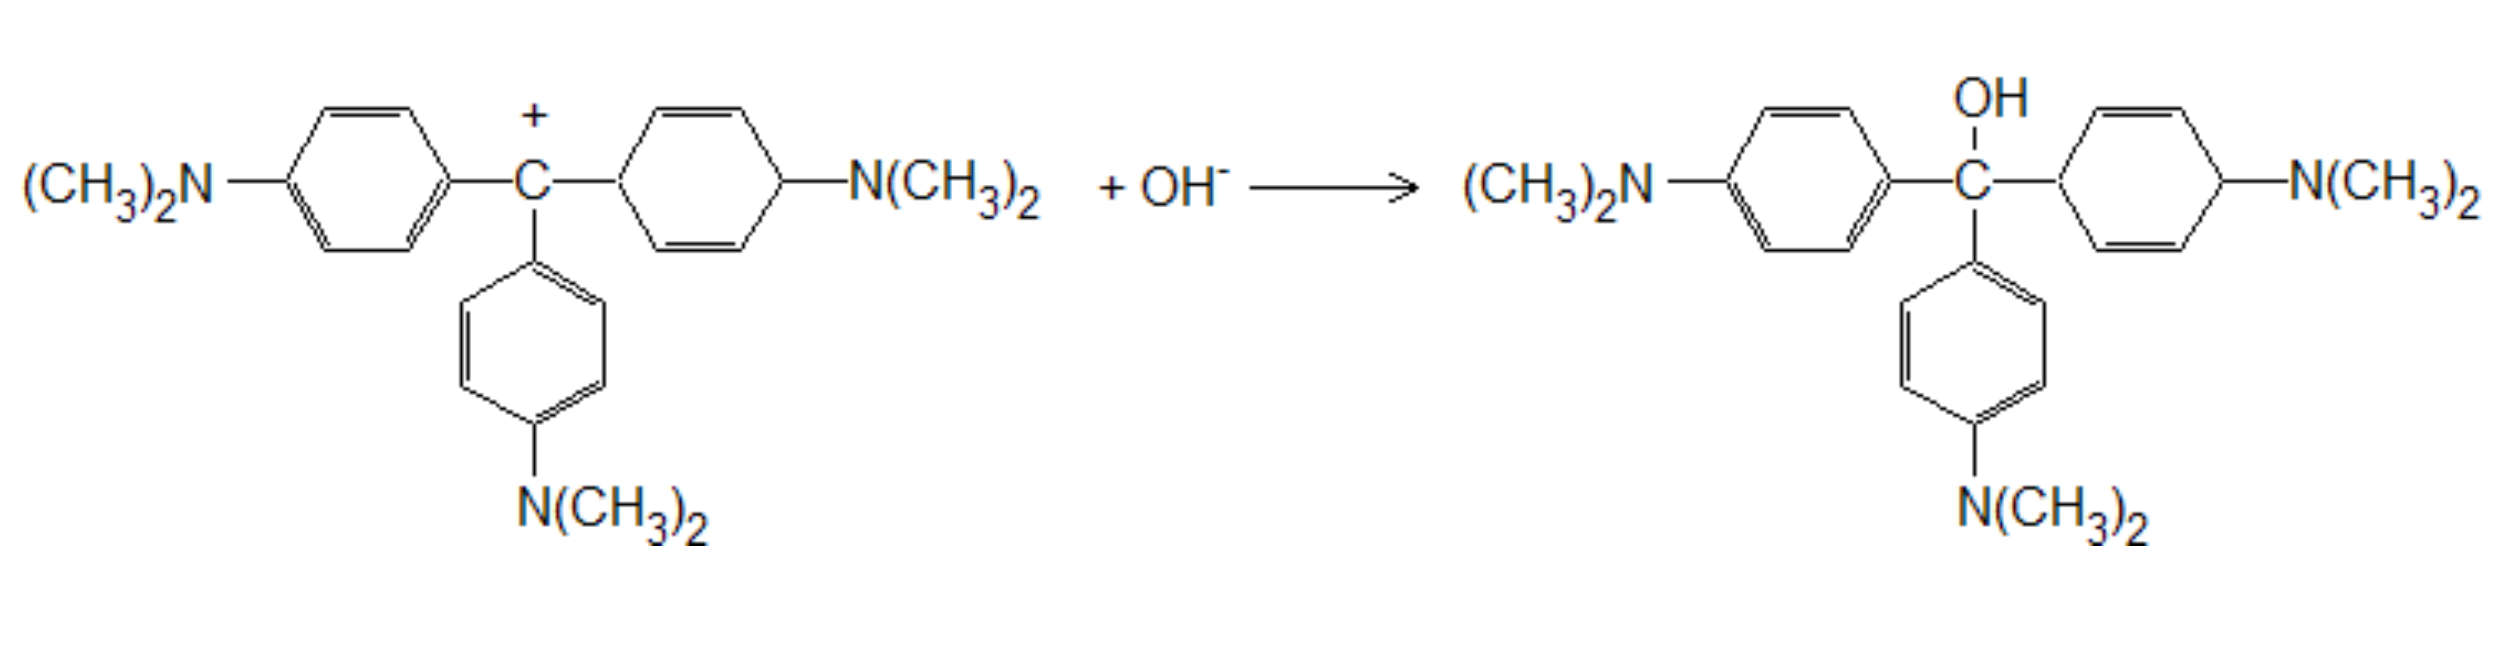
\includegraphics[scale=0.5]{Structural formula.png}
\caption{Structural formula equation}
\label{fig:Structural formula equation}
\end{figure}
\begin{equation}
\ce{CV+} + \ce{OH-} → \ce{CVOH}
\end{equation}


\section{Materials and Method}
\subsection{Materials}
The materials used in this lab are listed as follows:\\
Spectrometer, Cuvettes, 100-1000μl pipets, beakers, 0.1M \ce{NaOH} solution, Crystal violet (\ce{CV}) solution, and distilled water.

\subsection{Method}

\subsubsection{Part 1: Determine Rate Order}
The rate law for the reaction between \ce{NaOH} and \ce{CV+} can be written as:
\begin{equation}
Rate=\mathbit{k[\ce{OH-}]^a [\ce{CV+}]^b}
\end{equation}
In the equation above, k is the rate constant; both a and b are the order of each reactant. By controlling the variable, we can find out the order for each reactant. In this experiment, we perform three trials to get the initial rate of the breakdown of \ce{CV} under different \ce{[CV]} and \ce{[NaOH]} by using the spectrometer to test its absorption. To determine the concentration, Beer’s law should be applied:
\begin{equation}
A=\epsilon lc
\end{equation}
In the equation above, A is the absorption, $\epsilon$ is the molar absorption constant at 565nm, which is \ce{CV}’s absorption peak with the limitation of the spectrometer, l is the path length of the solution that light passes and c is the concentration of absorbing species.
\begin{table}[h!]
\centering
\begin{tabular}{||c c c c c||}
 \hline
 Trial No. & \ce{CV} (ml) & \ce{NaOH} (ml) & Water (ml) & Total (ml) \\ [0.5ex] 
 \hline\hline
 1 & 0.5 & 0.5 & 1.0 & 2.0 \\ 
 2 & 1.0 & 1.0 & 0.0 & 2.0 \\
 3 & 1.0 & 0.5 & 0.5 & 2.0 \\ [1ex] 
 \hline
\end{tabular}
\caption{Volume of each compound in each trial}
\label{table:1}
\end{table}

\subsubsection{Part 2: Determine k for [\ce{CV+}] by Using Linear Approximation}
In this experiment, the \ce{[NaOH]} is much greater than the \ce{[CV+]} we use. Therefore we can consider [\ce{OH-}] as the reactant won’t change a lot during the reaction, then the rate law can be simplified as:
\begin{equation}
 Rate=\mathbit{k[\ce{OH-}]^a[\ce{CV+}]^b \approx k’[\ce{CV+}]^b}
\end{equation}
As the order of \ce{CV-} has been determined in Part 1, integrated rate law can be applied to find k' for \ce{CV+} by changing [CV+]. If \ce{CV+} is in the first order, its concentration change should fit:
\begin{equation}
ln[\ce{CV+}] = ln[\ce{CV+}]_{0} - k't
\end{equation}

\subsubsection{Part 3: Determine Rate Constant k}
By applying the following equation:
\begin{equation}
k = k’/[\ce{OH}]_{0}^a
\end{equation}
We can determine the final rate constant k; the k here should be the average number of three trials.

\section{Result}
Changing in [\ce{CV+}] in three trials are shown as the following graphs. The Absorption (A) of \ce{CV+} has been transferred into the concentration of \ce{CV+} by applying Beer’s law.
\subsection{Concentration of \ce{CV+} vs Time}
\begin{figure}[H] 
\centering
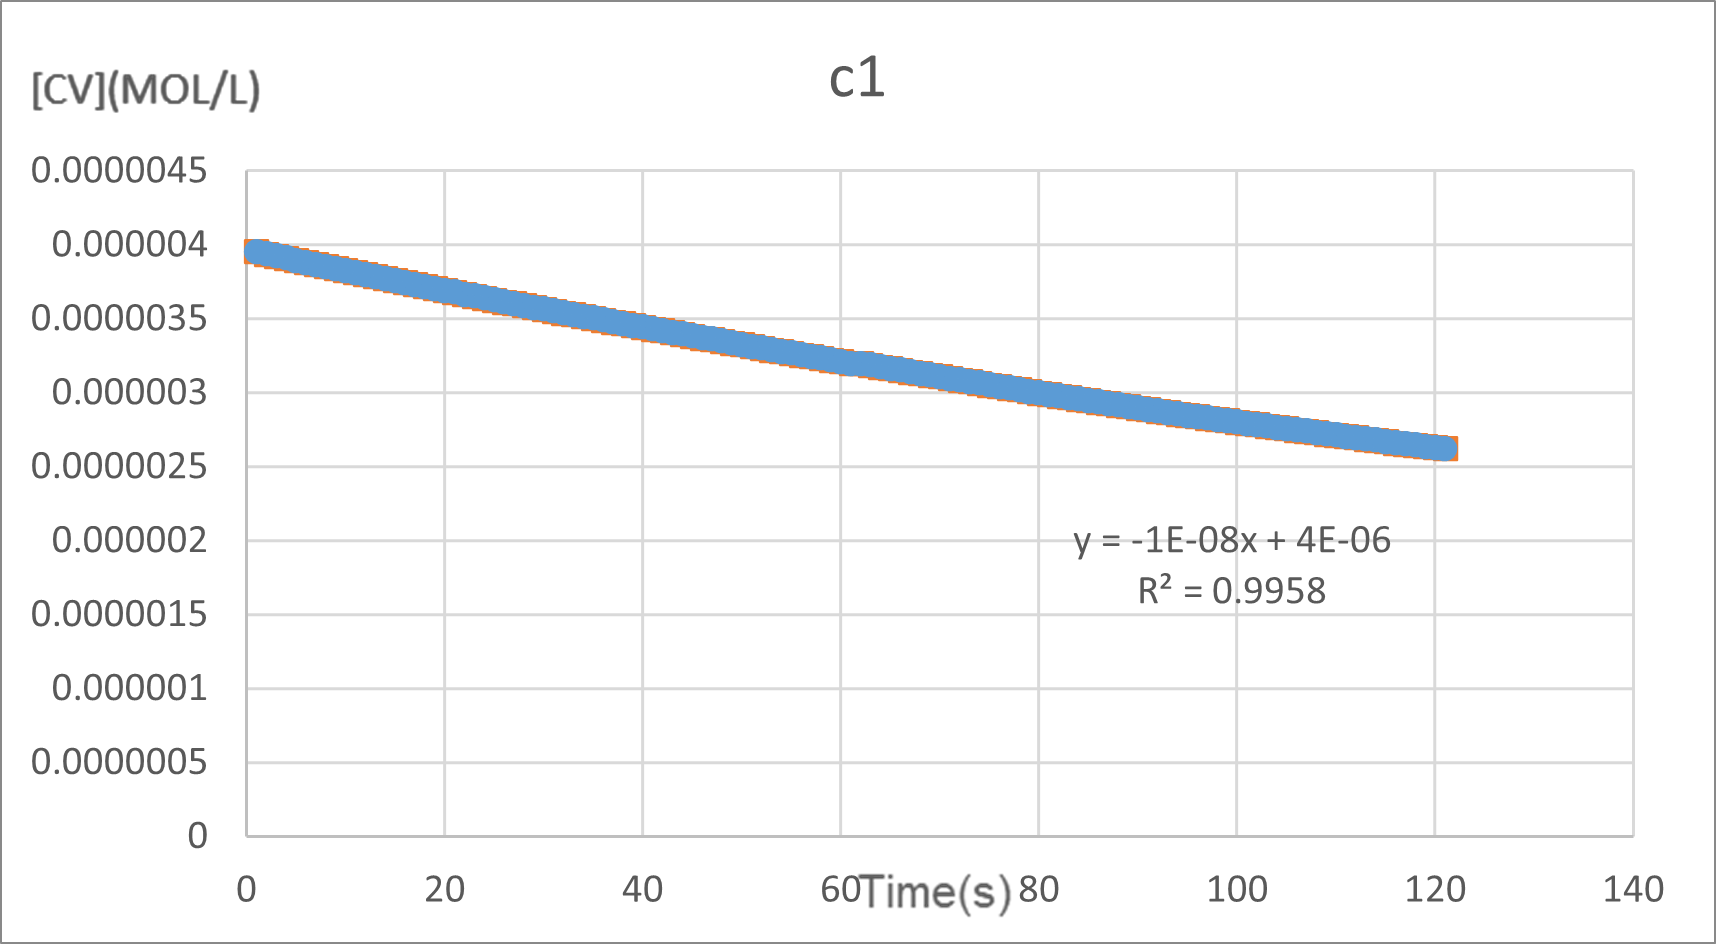
\includegraphics[scale=0.9]{c1.png}
\caption{trial 1: concentration of \ce{CV+} vs. time}
\end{figure}
\begin{figure}[H] 
\centering
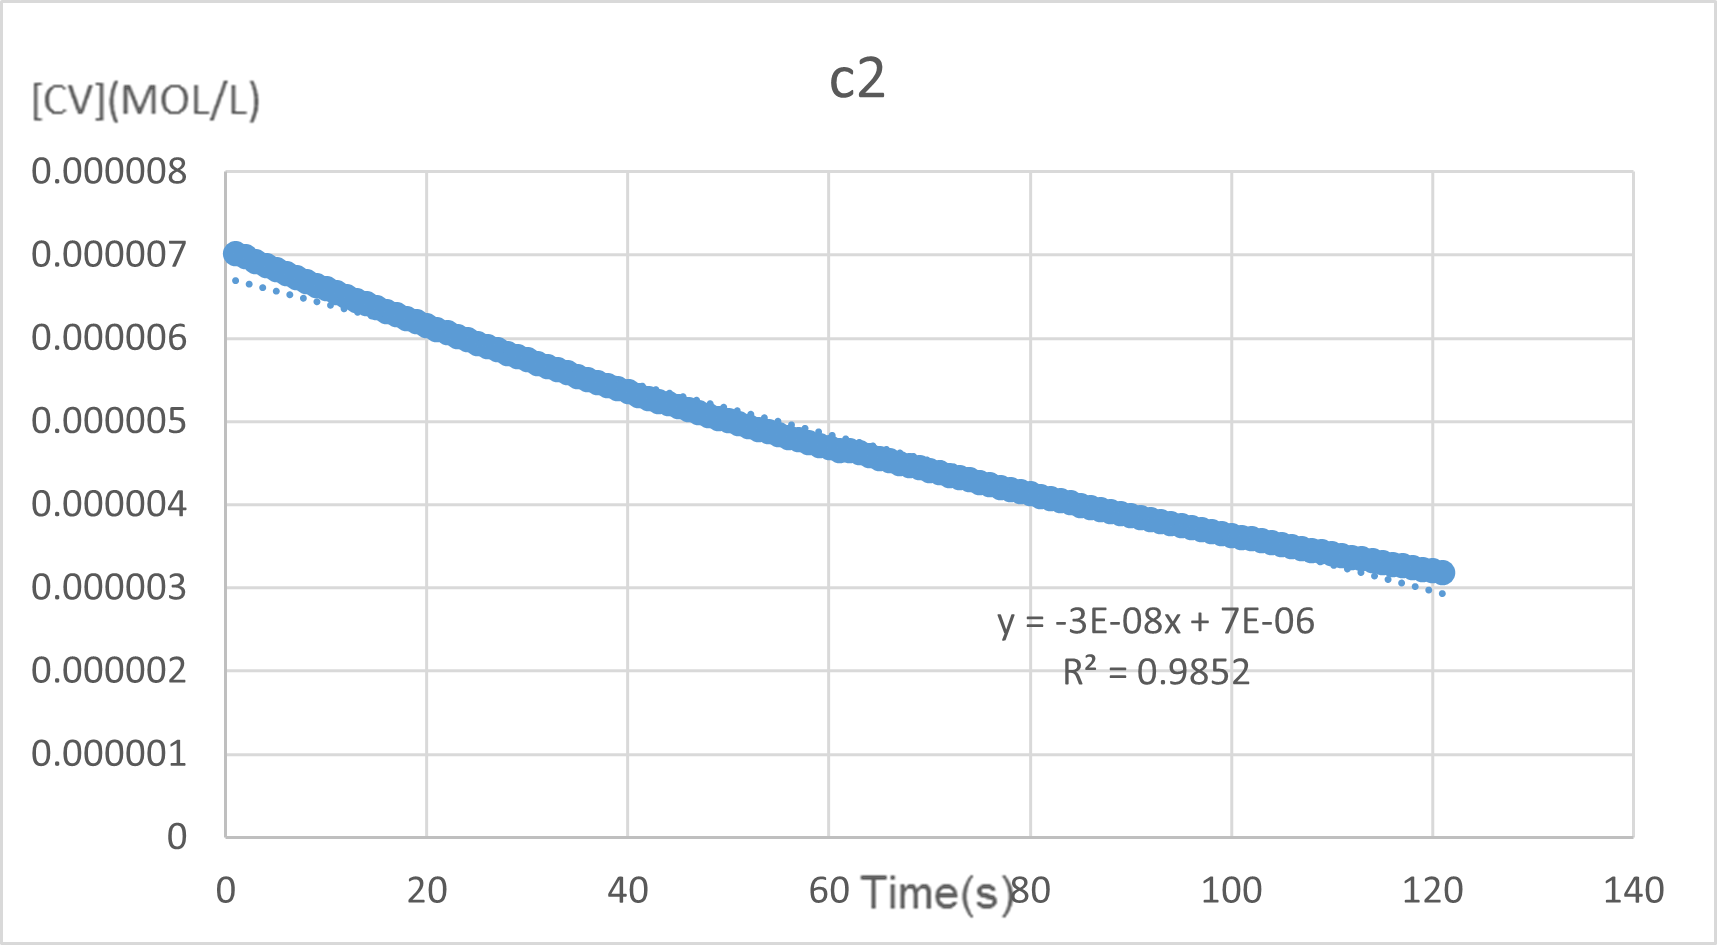
\includegraphics[scale=0.9]{c2.png}
\caption{trial 2: concentration of \ce{CV+} vs. time}
\end{figure}
\begin{figure}[H] 
\centering
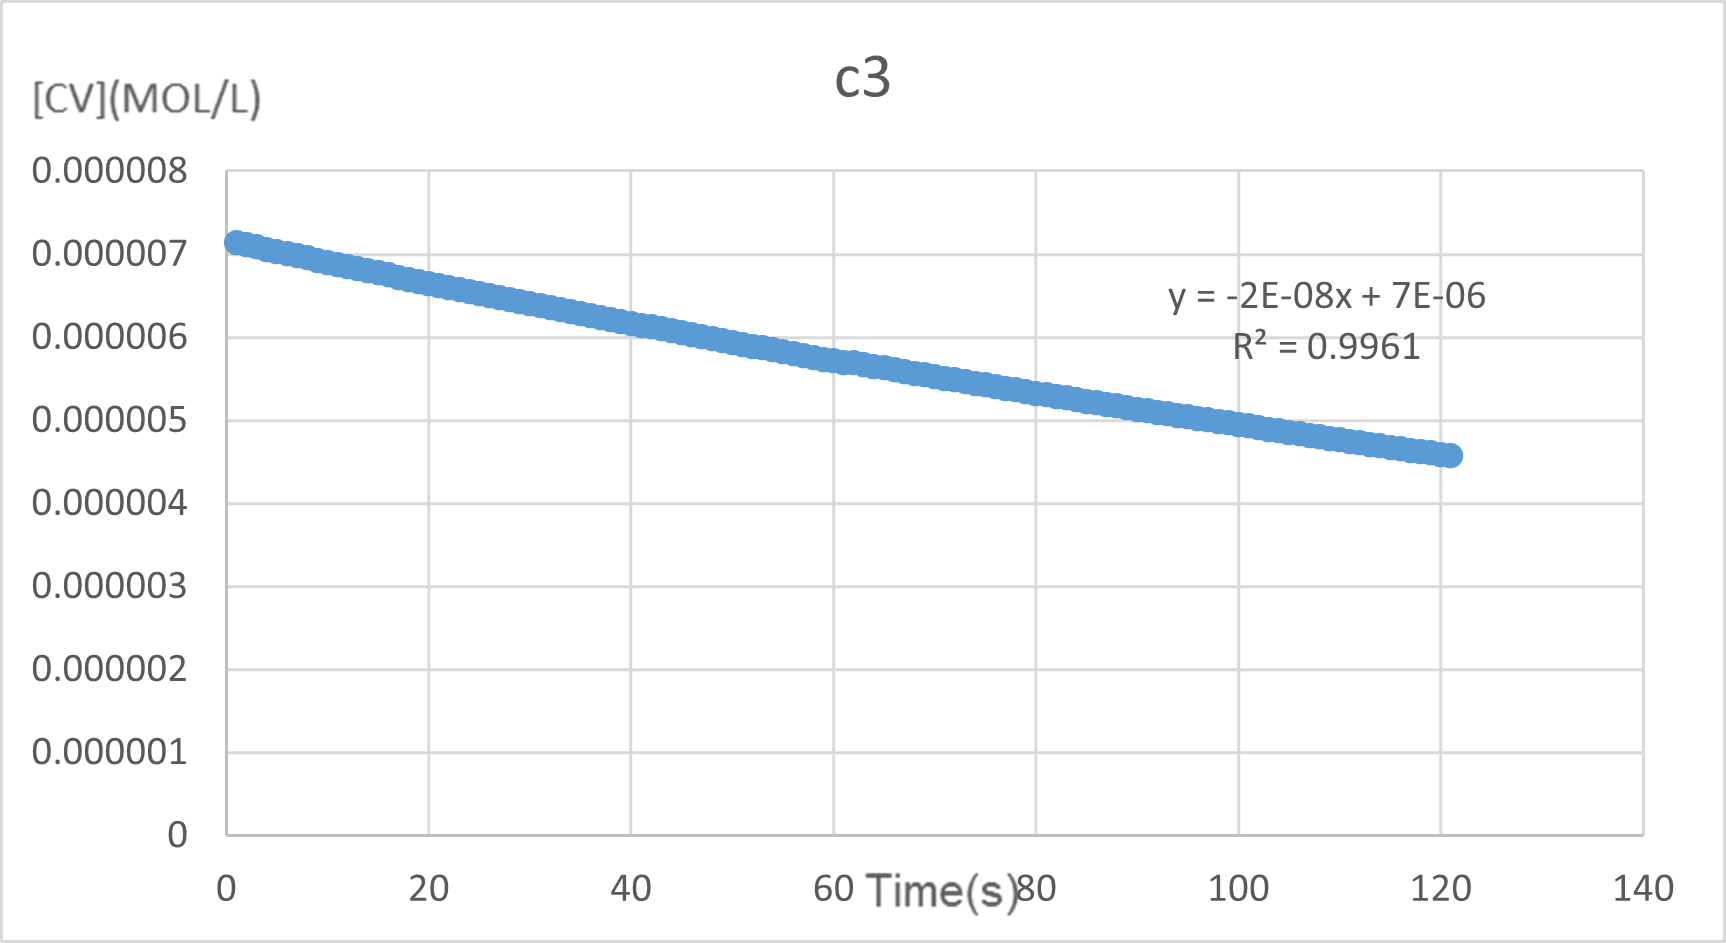
\includegraphics[scale=0.9]{c3.png}
\caption{trial 3: concentration of \ce{CV+} vs. time}
\end{figure}
The average $\mathbit{R^2}$ for [\ce{CV+}] vs time is 0.989

\subsection{Natural Logarithm of Concentration of \ce{CV+} vs Time}
\begin{figure}[H] 
\centering
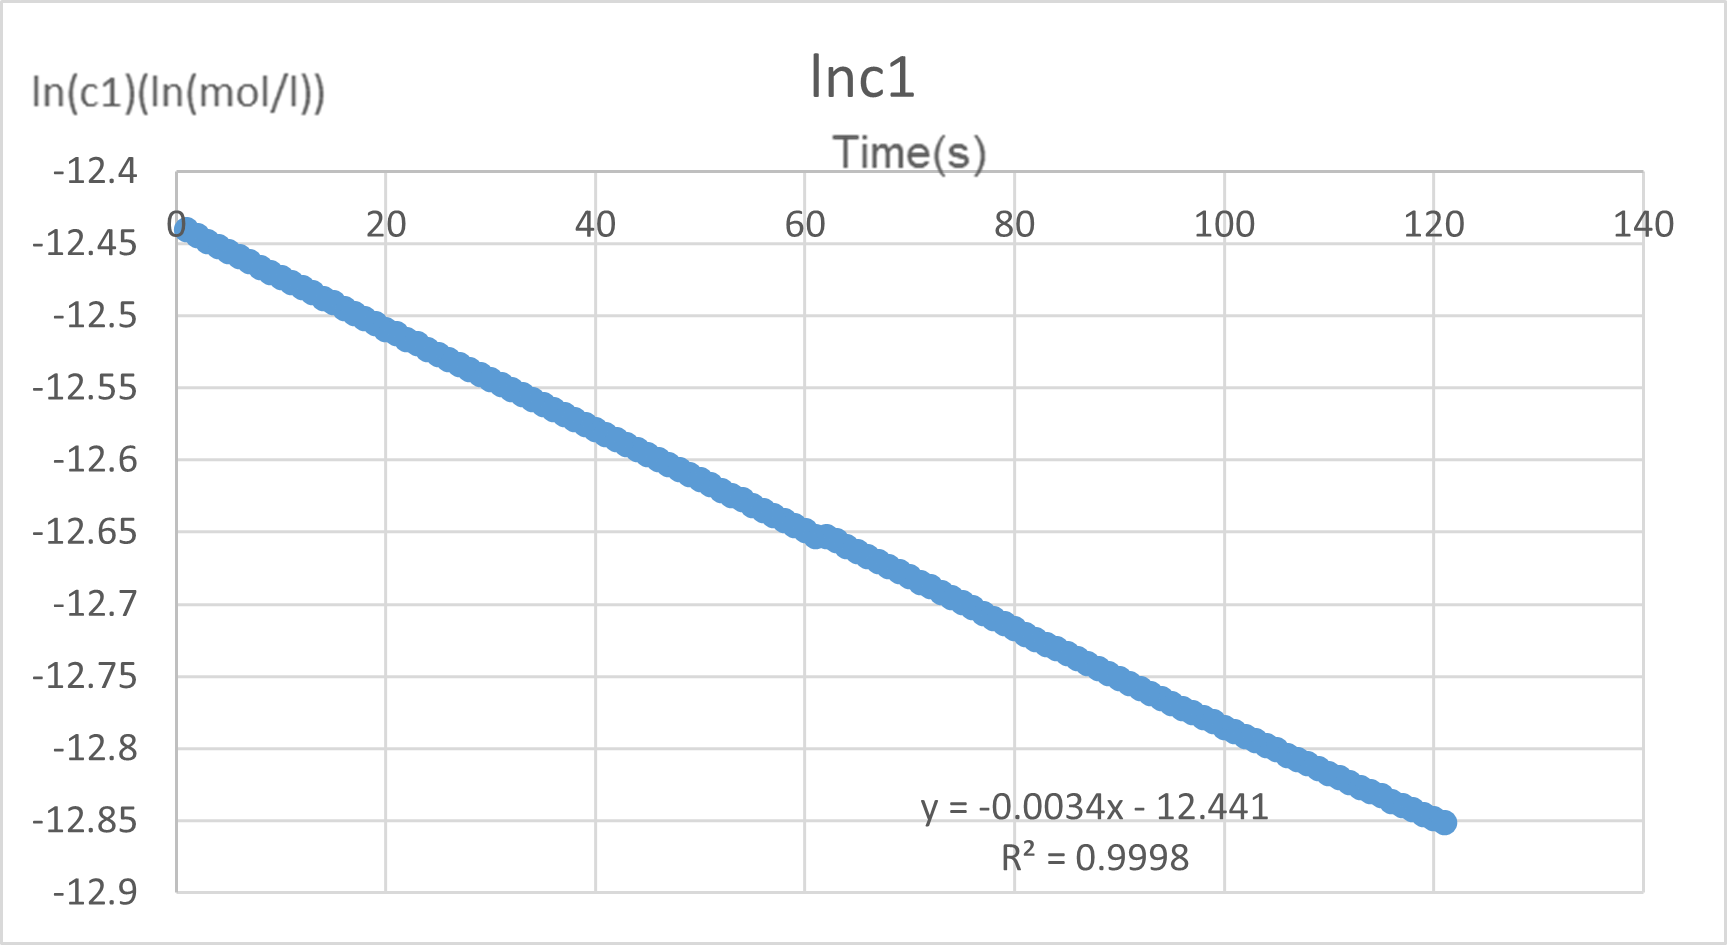
\includegraphics[scale=0.9]{lnc1.png}
\caption{trial 1: ln[\ce{CV+}] vs. time}
\end{figure}
\begin{figure}[H] 
\centering
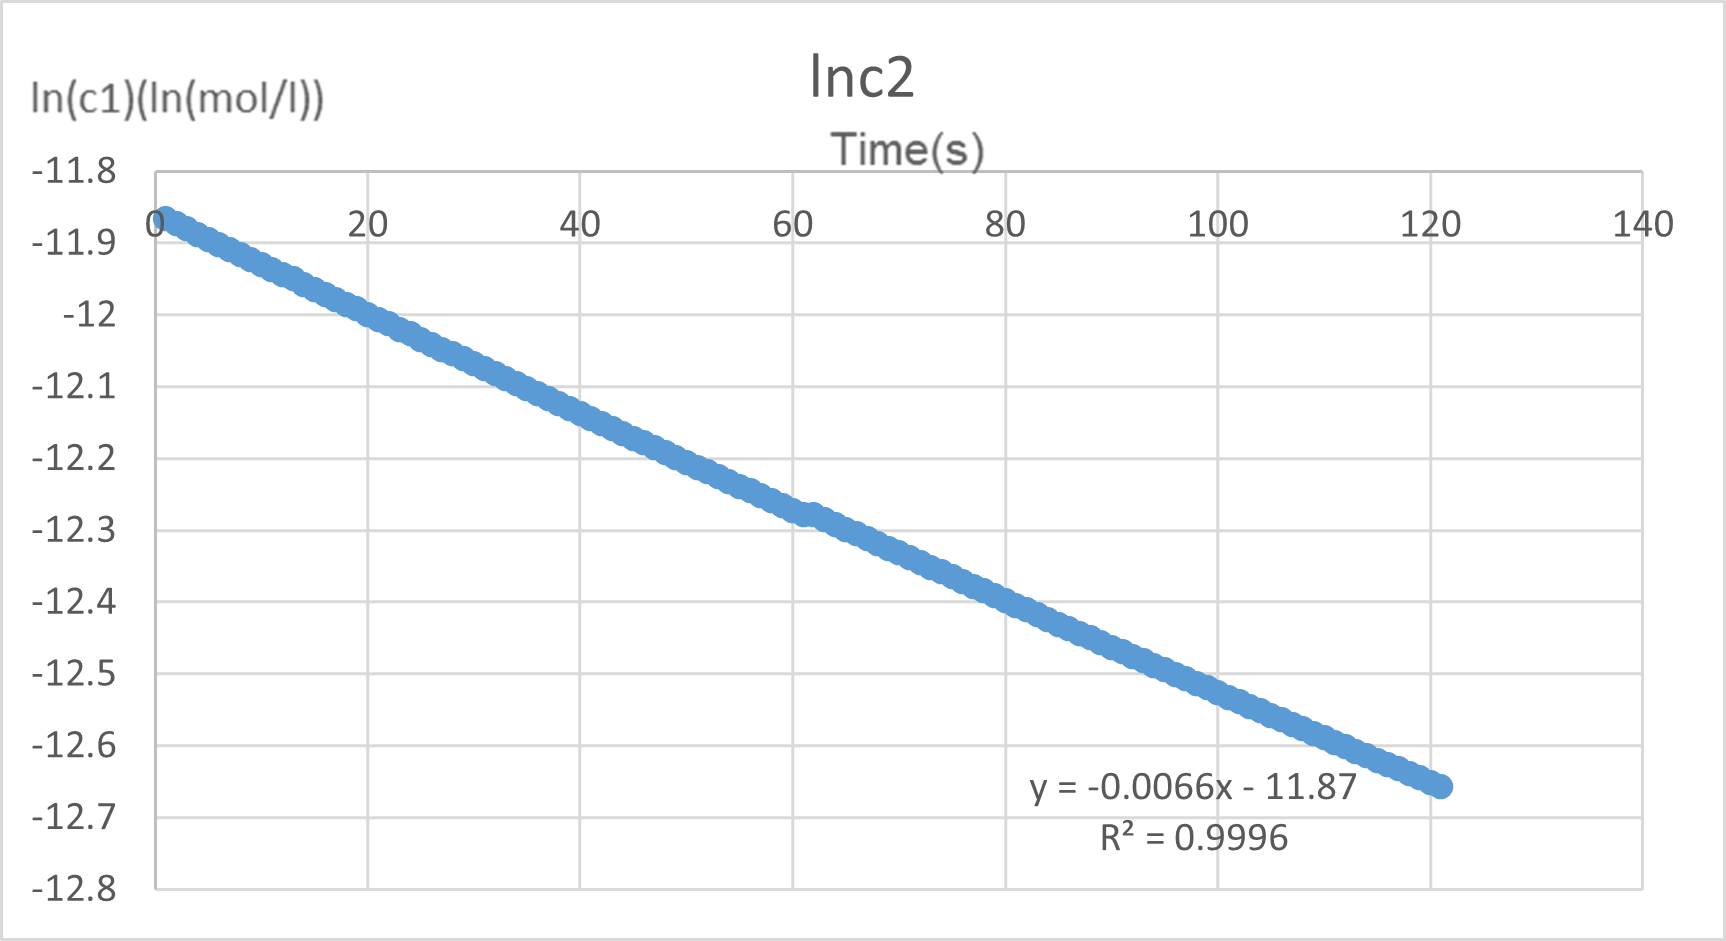
\includegraphics[scale=0.9]{lnc2.png}
\caption{trial 2: ln[\ce{CV+}] vs. time}
\end{figure}
\begin{figure}[H] 
\centering
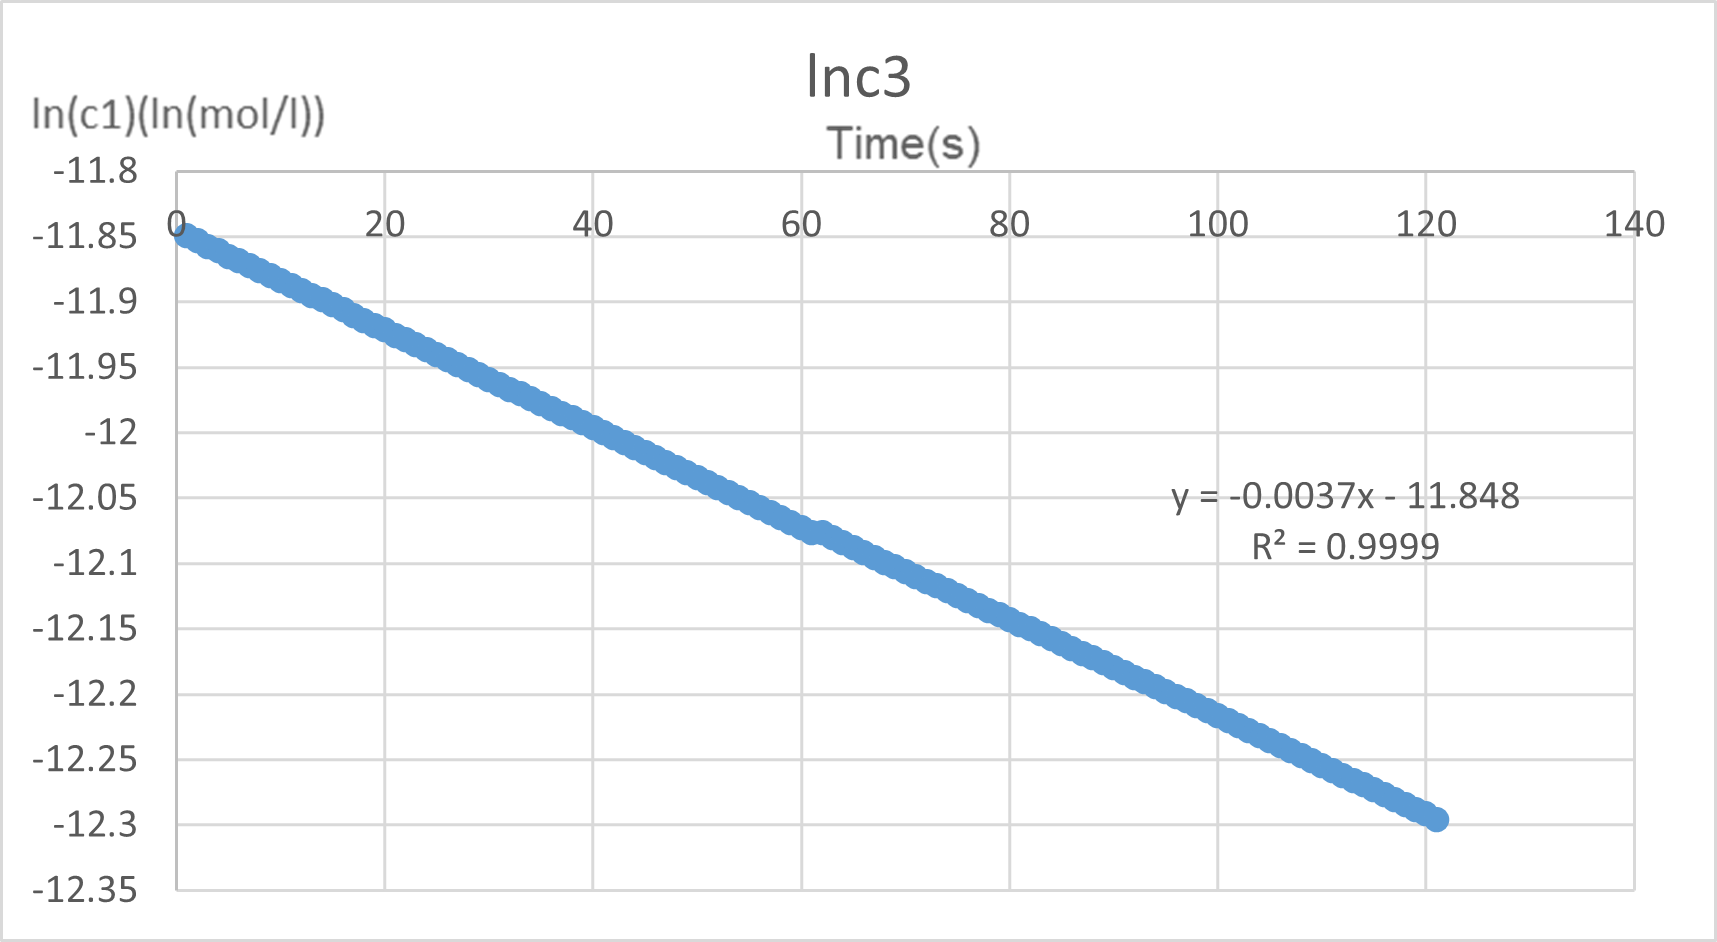
\includegraphics[scale=0.9]{lnc3.png}
\caption{trial 3: ln[\ce{CV+}] vs. time}
\end{figure}
The average $\mathbit{R^2}$ for ln[\ce{CV+}] vs time is 0.997

\subsection{Inverse of Concentration of \ce{CV+} vs Time}
\begin{figure}[H] 
\centering
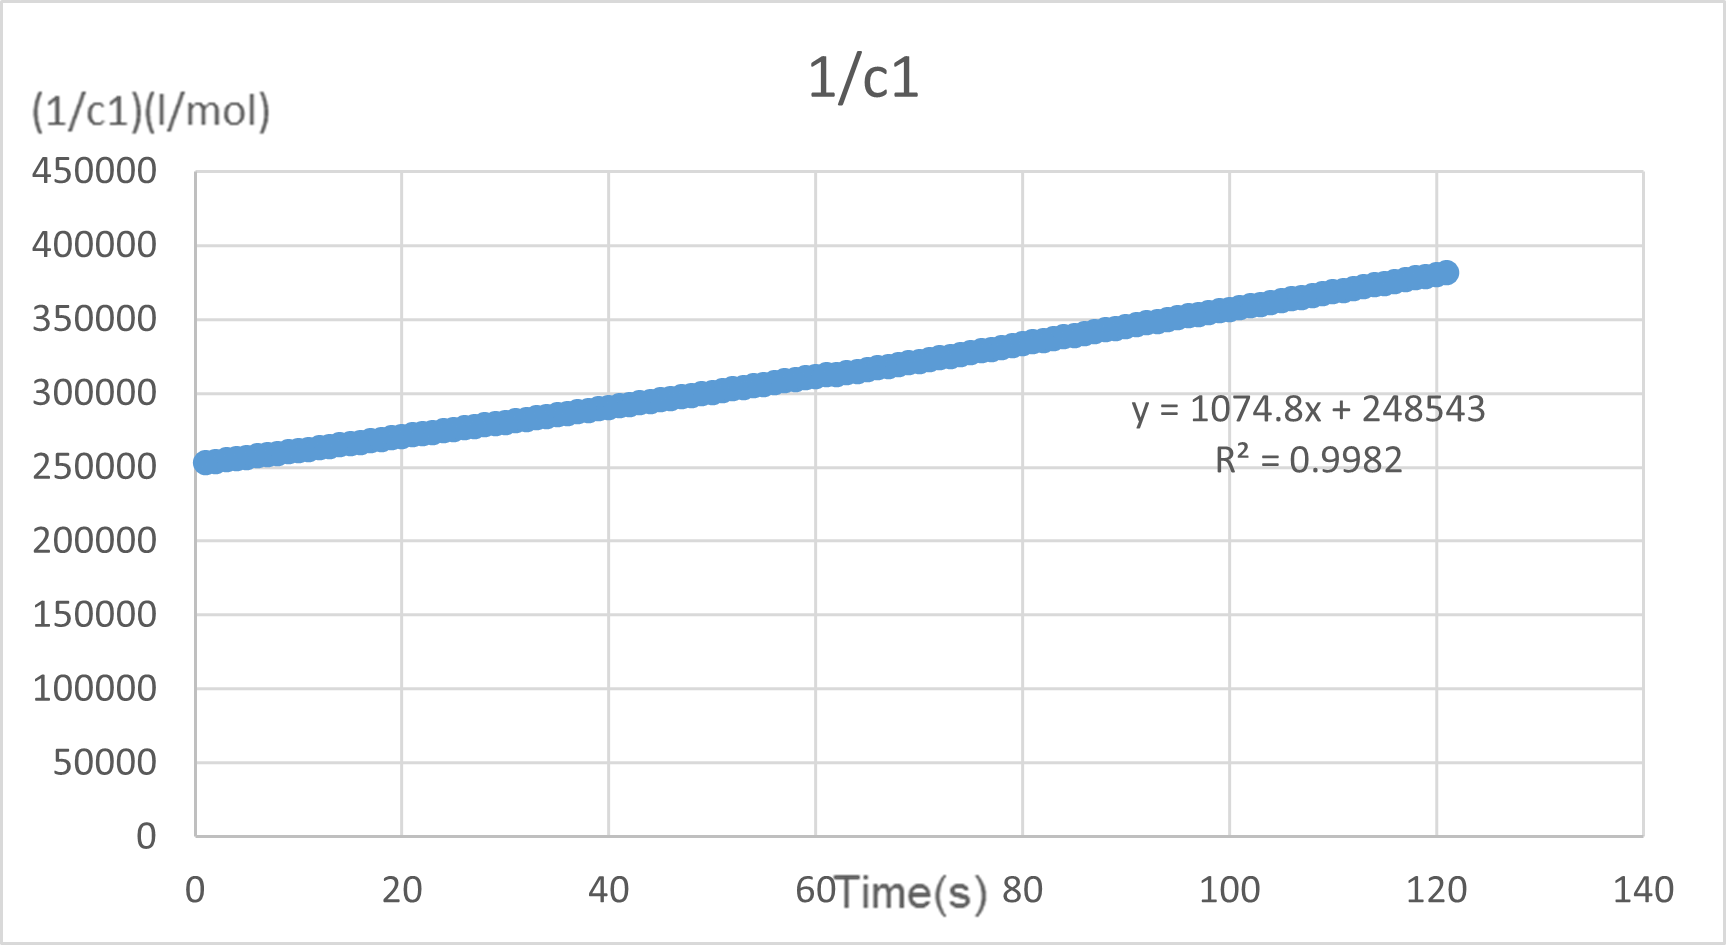
\includegraphics[scale=0.9]{1.png}
\caption{trial 1: 1/[\ce{CV+}] vs. time}
\end{figure}
\begin{figure}[H] 
\centering
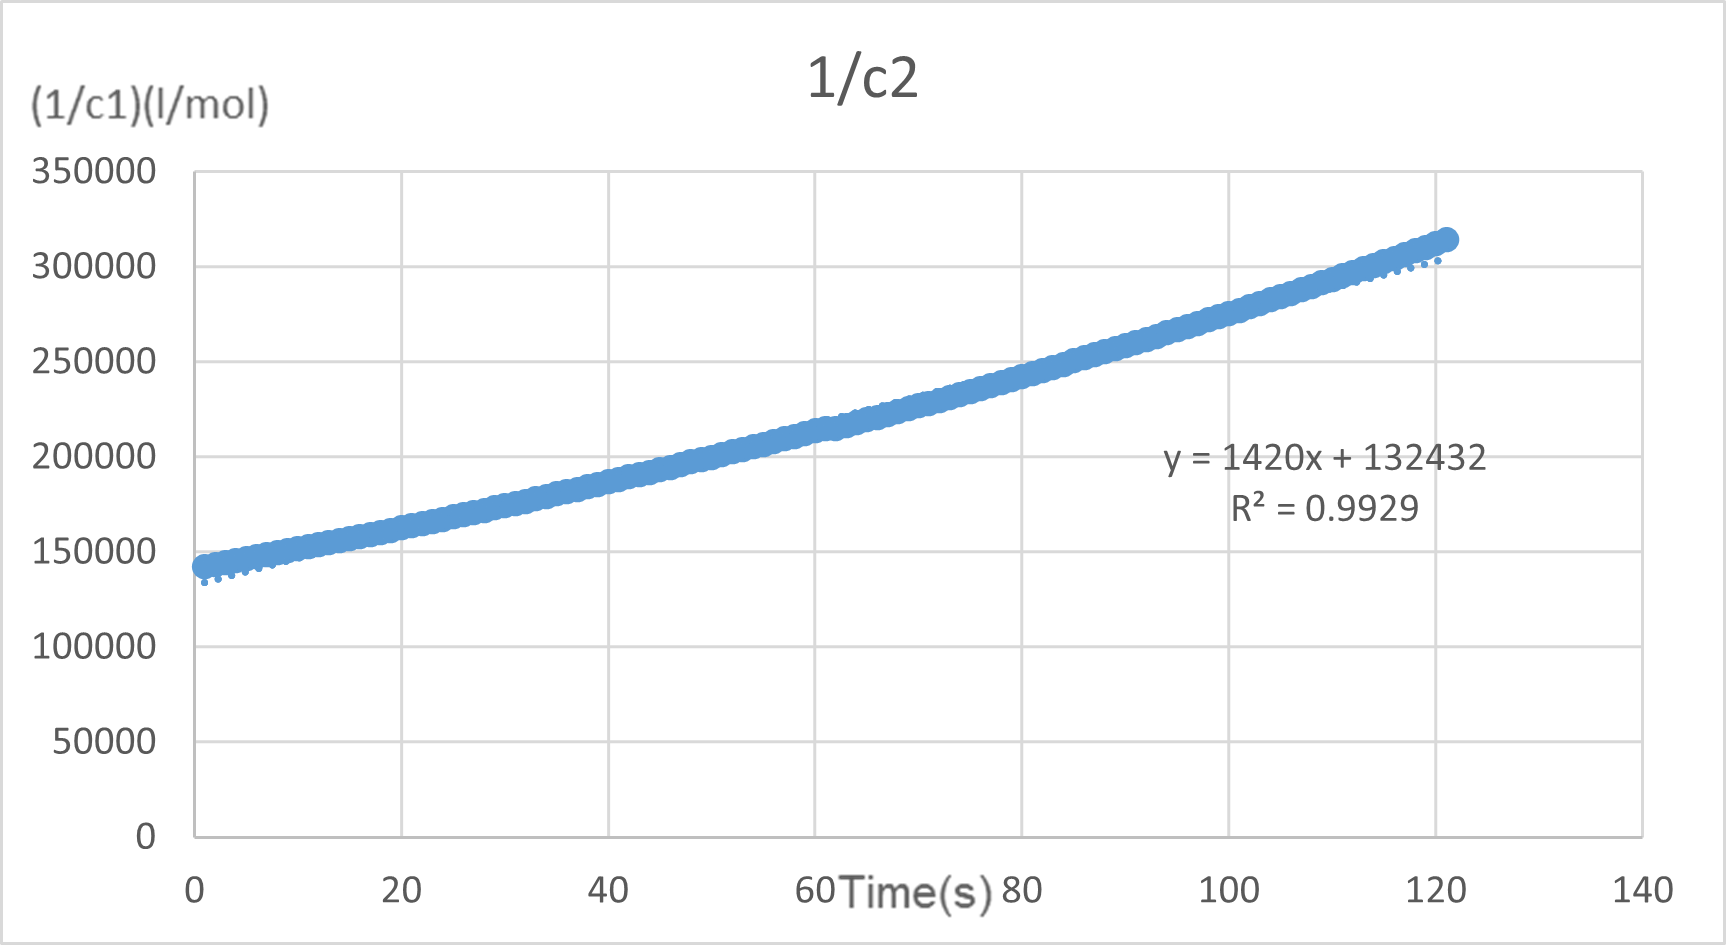
\includegraphics[scale=0.9]{2.png}
\caption{trial 2: 1/[\ce{CV+}] vs. time}
\end{figure}
\begin{figure}[H] 
\centering
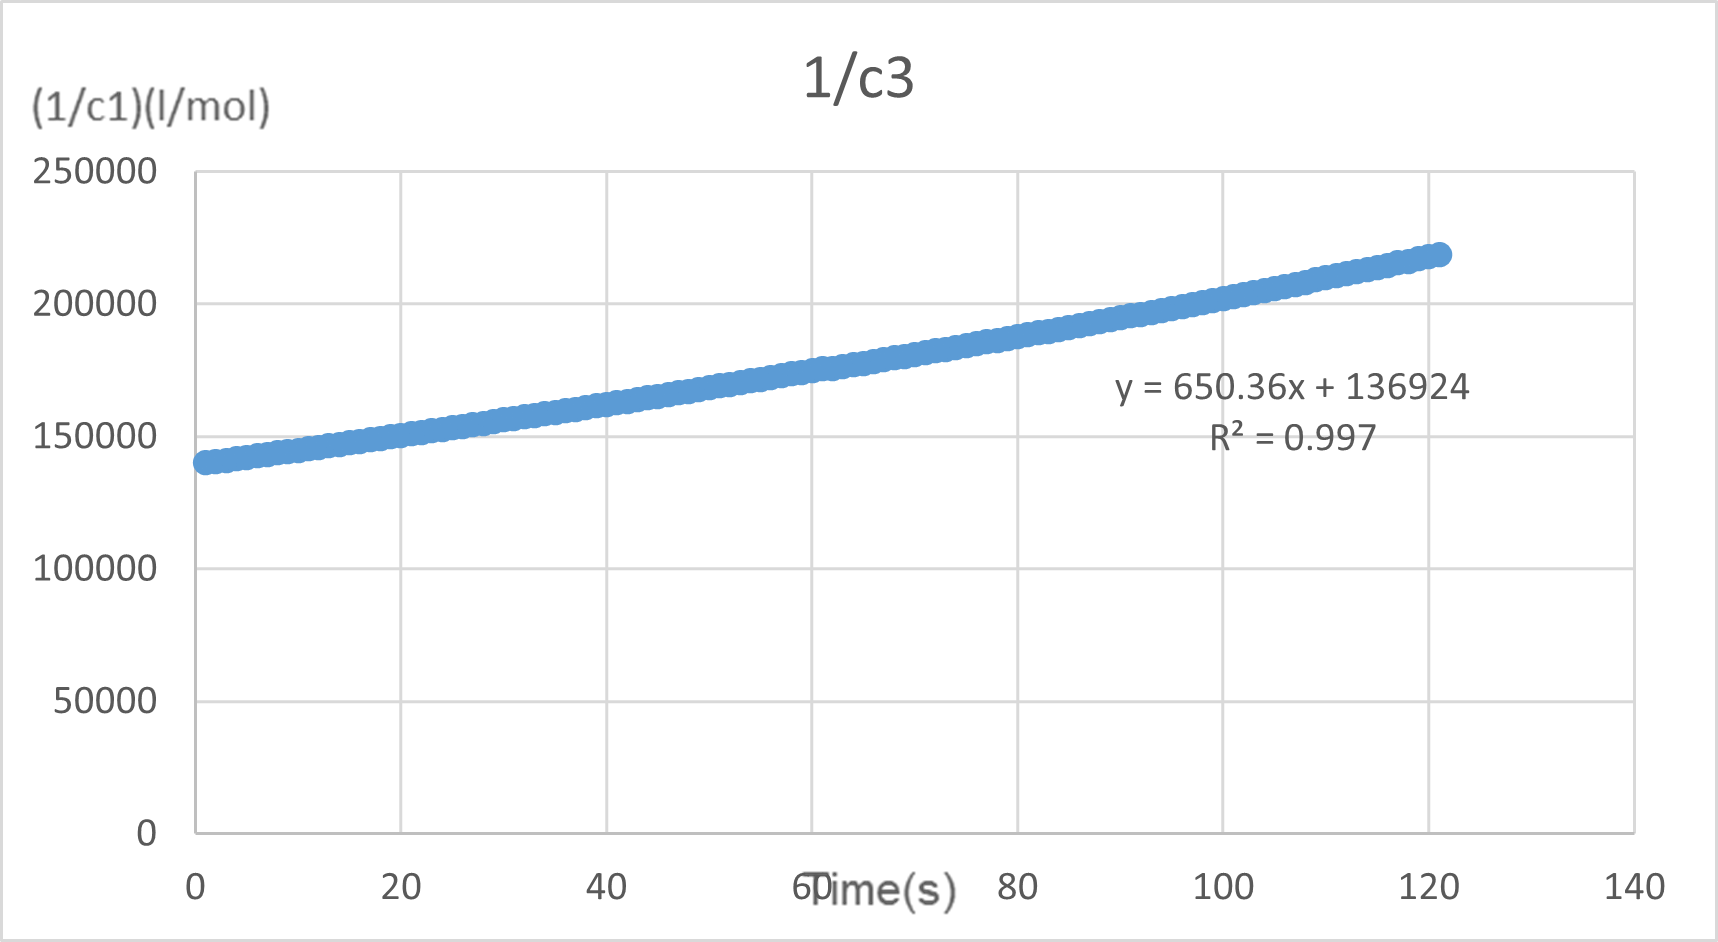
\includegraphics[scale=0.9]{3.png}
\caption{trial 2: 1/[\ce{CV+}] vs. time}
\end{figure}
The average $\mathbit{R^2}$ for ln[\ce{CV+}] vs time is 0.995\\
By the graphs, we can calculate that [\ce{CV+}] is in the first order as the average $\mathbit{R^2}$ for [\ce{CV+}] vs. time is 0.989, which is the highest among all and shows the linear relationship is the strongest.

\newpage
\section{Discussion}
The following equation can be computed from equation(1):
\begin{equation}
\frac{\mathbit{Rate}(\mathbit{Trial}\ \mathbf{1})}{\mathbit{Rate}(\mathbit{Trial}\ \mathbf{3})}=\frac{\mathbf{k[OH-]^a(Trial 1)[CV+]^b(Trial 1)}}{\mathbf{k[OH-]^a(Trial 3)[CV+]^b(Trial 3)}}
\end{equation}
The change of [\ce{CV+}] in the graph (2), (3), and (a) is approximately linear, so we can assume the rate to be the slope of the line. We also know that k is a constant; the difference between trial 1 and trial 3 is small that the concentration of [\ce{OH-}] doubles in trial 3. As a result, the following equation can be determined:
\begin{equation}
\frac{-\mathbf{1}\mathbit{E}-\mathbf{08}}{-\mathbf{2}\mathbit{E}-\mathbf{08}}={(\frac{\mathbf{1}}{\mathbf{2}})}^\mathbit{a}=\mathbf{0}.\mathbf{5}
\end{equation}
In this case, a=1 suits the equation well.
Similarly, by using Trial 2 and Trial 3 and following the same step.
\begin{equation}
\frac{-\mathbf{2}\mathbit{E}-\mathbf{08}}{-\mathbf{3}\mathbit{E}-\mathbf{08}}={(\frac{\mathbf{1}}{\mathbf{2}})}^\mathbit{b}=\mathbf{0}.\mathbf{67}
\end{equation}
In this case, b=1 also suits the equation well.
The rate law is hereby determined:
\begin{equation}
Rate=k[\ce{CV+}][\ce{OH-}]
\end{equation}
By the graphs above, we can calculate that [\ce{CV+}] is in the first order as the average $\mathbit{R^2}$ for [\ce{CV+}] vs. time is 0.989, which is the highest among all and shows the linear relationship is the strongest. The following table shows the outcome of this experiment.
\begin{table}[h!]
\centering
\begin{tabular}{||c c c c ||}
 \hline
 Trial No. & K’ (1/s) & [\ce{OH-}]_{0}(mol/l) & k(l/mol*s) \\ [0.5ex] 
 \hline\hline
 1 & 0.0034 & 5*{\mathbf{10}}^{-\mathbf{5}} & 68 \\ 
 2 & 0.0066 & 1*{\mathbf{10}}^{-\mathbf{4}} & 66 \\
 3 & 0.0037 & 5*{\mathbf{10}}^{-\mathbf{5}} & 74 \\ [1ex] 
 \hline
\end{tabular}
\caption{Rate Constant in each Trial}
\label{table:1}
\end{table}
The average rate constant in this experiment is 70

\section{Conclusion}
In this experiment, we use the spectrometer to determine absorption to determine the [\ce{CV+}] and [\ce{OH_}]. Moreover, excel is used to plot the graphs. Calculate the rate
constant for the reaction. After completing this experiment, my knowledge about kinetics was expanded, and I learned how to do basic data analysis and write a laboratory report.

\section{References}
[1] Chemistry Lab Manual 2020 Spring, NYU Shanghai

\end{document}
